% Classe, package, etc. 
% L'option ``compress'' dans le documentclass permet d'avoir une table
% des matières compressée en haut des transparents
\documentclass[a4paper,compress]{beamer}  %  [handout]{beamer}

%\mode<presentation>{\usetheme{Hannover}}
\usepackage[francais]{babel}
\usepackage[utf8]{inputenc}
\usepackage[T1]{fontenc}
% \usepackage{lmodern}
%\usepackage[english]{babel}
% \usepackage[babel]{microtype}
\usepackage{xcolor,colortbl}
\usepackage{graphicx,url}
\usepackage{enumerate}
\usepackage{amssymb,amsthm}
\usepackage{times}
%\usepackage{amsmath,amscd}
\usepackage[all]{xy}
%\usepackage{soul} % pour barrer du texte
\usepackage{url}\urlstyle{same}
\usepackage{marvosym} % Pour les euros

% Automatic import of SVG, replacing text with LaTeX
% Compile with: (pdf)latex -shell-escape ...
\newcommand{\executeiffilenewer}[3]{%
\ifnum\pdfstrcmp{\pdffilemoddate{#1}}%
{\pdffilemoddate{#2}}>0%
{\immediate\write18{#3}}\fi%
}
\def\svgmode{ps}\ifx\pdfoutput\undefined
\def\executeiffilenewer#1#2#3{\immediate\write18{#3}}\else%\bibliography{bibli}

\ifnum\pdfoutput<1\else\def\svgmode{pdf}\fi\fi
\newcommand{\includesvgX}[1]{%
\executeiffilenewer{#1.svg}{#1.\svgmode}%
{inkscape -z -D --file=#1.svg --export-latex %
--export-\svgmode=#1.\svgmode}%
\input{#1.\svgmode_tex}%
}
\newcommand{\includesvg}[2][]{%
\def\tempa{#1}\def\tempb{}%
\ifx\tempa\tempb\else\let\svgwidth\tempa\fi
\includesvgX{\svgpath#2}%
}



%%%%%%%%%%%%%%%%%%%%%%%%%%%%%%%%%%%%%%%%%%%%%%%%%%%%%%%%%%%%%%%%%%%%%%%%%%
% A few shortcuts..
\def\scal#1{\hbox{\rm#1}}
\def\vect#1{\hbox{\bf#1}}
\def\Real{{\rm I\hskip-2pt R}}
\def\Integer{{\rm Z\hskip-4pt Z}}
\def\sus#1{{\hbox{\scriptsize #1}}}

\def\derivOne#1#2{{\scal d#1 \over \scal d#2}}
\def\derivTwo#1#2{{\scal d^2#1 \over \scal d#2^2}}
\def\partialOne#1#2{{\partial#1 \over \partial#2}}
\def\partialTwoSame#1#2{{\partial^2#1 \over \partial#2^2}}
\def\partialTwo#1#2#3{{\partial^2#1 \over \partial#2\,\partial#3}}
\def\partialThree#1#2#3#4{{\partial^3#1
 \over \partial#2\, \partial#3\, \partial#4}}
\def\partialThree_TwoOne#1#2#3{{\partial^3#1 \over \partial#2^2\, \partial#3}}
\def\partialThree_OneTwo#1#2#3{{\partial^3#1 \over \partial #2\, \partial#3^2}}
\def\partialThreeSame#1#2{{\partial^3#1 \over \partial#2^3}}

\def\inprod#1#2{\langle#1, #2\rangle}
% ---- DELIMITER PAIRS ---- from Jeff Erickson
\def\floor#1{\lfloor #1 \rfloor}
\def\ceil#1{\lceil #1 \rceil}
\def\seq#1{\langle #1 \rangle}
\def\set#1{\{ #1 \}}
\def\abs#1{\mathopen| #1 \mathclose|}	% use instead of $|x|$ 
\def\norm#1{\mathopen\| #1 \mathclose\|}	% use instead of $\|x\|$ 
\def\indic#1{\big[#1\big]}                              % indicator variable; Iverson notation
					                                % e.g., Kronecker delta = [x=0]
\def\dual#1{{#1}^{\Delta}}
\def\bidual#1{{#1}^{\Delta\Delta}}

\newcommand{\ematrix}{\end{array}\right)}
\newcommand{\Alpha}{\mbox{\bf \LARGE $\alpha$}}
\newcommand{\Kappa}{\mbox{\bf \LARGE $\kappa$}}
\newcommand{\degr}{$\!\!^\circ$}
% \newcommand{\Z}{\mbox{\rm Z\hskip-4pt Z}}
\newcommand{\Z}{\mathbb{Z}}
%\newcommand{\N}{\mbox{\rm I\hspace{-.2em}N}}
\newcommand{\N}{\mathbb{N}}
\newcommand{\Reel}{\mbox{\rm I\hspace{-.2em}R}}
                %%  ATTENTION ne pas retirer les espaces dans \Complex !!!
\newcommand{\R}{\mathbb{R}}
% \newcommand{\R}{\mbox{\rm I\hspace{-.2em}R}}
                %%  ATTENTION ne pas retirer les espaces dans \Complex !!!
\newcommand{\C}{\mathbb{C}}
%\newcommand{\C}{\mbox{ \rm \rule[.05ex]{.15ex}{1.4ex}\hspace{-1.4ex} C}}
\newcommand{\Complex}{\mbox{ \rm \rule[.05ex]{.15ex}{1.4ex}\hspace{-1.4ex} C}}
\newcommand{\Q}{\mathbb{Q}}
\providecommand{\1}{\mbox{\rm 1\hspace{-.27em}I}}
\newcommand{\0}{\mbox{\rm I\hspace{-.45em}}\mathbf{0}}
\newcommand{\zbf}{\mathbf{0}}

%% \newcommand{\binom}[2]{\left(\!\!\!\begin{array}{c} #1 \\
%% #2\end{array}\!\!\!\right)}
        %% binom d�fini dans amsmath
\newcommand{\matundeux}[2]{\left[\!\!\!\begin{array}{c} #1 \\
     #2\end{array}\!\!\!\right]}

\newcommand{\matuntrois}[3]{\left[\!\!\!\begin{array}{c} #1 \\
     #2 \\ #3\end{array}\!\!\!\right]}
%% \newcommand{\implies}{\Rightarrow} 
        %% implies d�fini dans amsmath
\newcommand{\isequ}{\Leftrightarrow}
\newcommand{\inter}[1]{\stackrel{\circ}{#1}}
\newcommand{\clos}[1]{\bar{#1}}
\newcommand{\complt}[1]{\complement{#1}}
\newcommand{\contract}{\mbox{/\hspace{-.2em}/}}
\newcommand{\inv}{\ensuremath{^{-1}}}
\newcommand{\onto}{\twoheadrightarrow}
\newcommand{\into}{\hookrightarrow}

\makeatletter\def\proof{\@ifnextchar[{\@xproof}{\@proof}}
\def\endproof{\unskip\kern 10\p@ \begingroup \unitlength\p@
  \linethickness{.4\p@} \framebox(6,6){} \endgroup \endtrivlist }
\def\@proof{\trivlist \item[ \hskip 10\p@ \hskip \labelsep {\sc
    Proof.}  ] \ignorespaces }
\def\@xproof[#1]{\trivlist \item[\hskip 10\p@\hskip \labelsep{\sc
    Proof #1.}] \ignorespaces } \makeatother

\makeatletter\def\skproof{\@ifnextchar[{\@xskproof}{\@skproof}}
\def\endskproof{\unskip\kern 10\p@ \begingroup \unitlength\p@
  \linethickness{.4\p@} \framebox(6,6){} \endgroup \endtrivlist }
\def\@skproof{\trivlist \item[ \hskip 10\p@ \hskip \labelsep {\sc
    Sketch of Proof.}  ] \ignorespaces }
\def\@skxproof[#1]{\trivlist \item[\hskip 10\p@\hskip \labelsep{\sc
    Sketch of Proof #1.}] \ignorespaces } \makeatother

\makeatletter\def\preuve{\@ifnextchar[{\@xpreuve}{\@preuve}}
\def\endpreuve{\unskip\kern 10\p@ \begingroup \unitlength\p@
  \linethickness{.4\p@} \hfill $\Box${} \endgroup \endtrivlist }
\def\@preuve{\trivlist \item[  {\bf
    Preuve :}  ] \ignorespaces }
\def\@xpreuve[#1]{\trivlist \item[\hskip \labelsep{\bf
    Preuve #1 :}] \ignorespaces } \makeatother

\makeatletter\def\skpreuve{\@ifnextchar[{\@xskpreuve}{\@skpreuve}}
\def\endskpreuve{\unskip\kern 10\p@ \begingroup \unitlength\p@
  \linethickness{.4\p@} \framebox(6,6){} \endgroup \endtrivlist }
\def\@skpreuve{\trivlist \item[ \hskip 10\p@ \hskip \labelsep {\sc
    Sketch of Preuve.}  ] \ignorespaces }
\def\@skxpreuve[#1]{\trivlist \item[\hskip 10\p@\hskip \labelsep{\sc
    Sketch of Preuve #1.}] \ignorespaces } \makeatother
%%% Local Variables: 
%%% mode: plain-tex
%%% TeX-master: "math_macros"
%%% End: 
 %% un $ pour le HOME

\def\deriv#1#2{{#1 \!\!\cdot\!\! #2}}


%%%%%%%%%%%%%%%%%%%%%%%%%%%%%%%%%%%%%%%%%%%%%%%%%%%%%%%%%%%%%%%%%%%%%%%%%%
% graphics
\graphicspath{{./}{github/}}
\def\svgpath{figures/}

%\DeclareGraphicsExtensions{.eps,.eps.gz}
%\DeclareGraphicsRule{.eps.gz}{eps}{.eps.bb}{`gunzip -c #1}

%-------------------------------------------------------------------------
% Thème des transparents
\usetheme{Warsaw} %{default}
%\usetheme{classic}
\setbeamercovered{invisible}

% pour le problème d'affichage du texte après les blocks
% \let\origframetitle\frametitle
% \renewcommand{\frametitle}[1]{%
%   \origframetitle{#1}\usebeamercolor*{normal text}%
% }
%---------------------------------------------------------------------------
% Il existe aussi des thèmes de couleurs
%\usecolortheme{crane}

%--------------------------------------------------------------------------
% Pour que seule la section courante apparaisse dans le bandeau de
% table des matières
%\setbeamertemplate{section in head/foot shaded}{}
%\setbeamertemplate{subsection in head/foot shaded}{}
\setbeamertemplate{footline}{}

%--------------------------------------------------------------------------
% Niveau de transparence des éléments grisés avant d'être affichés 
\beamertemplatetransparentcoveredmedium

%-------------------------------------------------------------------------
% Définitions de couleurs
\definecolor{vert}{rgb}{0,255,0}
\definecolor{darkgreen}{rgb}{0,0.3,0}
\definecolor{rouge}{rgb}{0.75,0,0}
\definecolor{lightblue}{rgb}{0,255,255}
\definecolor{myorange}{RGB}{255,165,0}
\definecolor{mauve}{rgb}{201,0,224}
\definecolor{kaki}{rgb}{0.13,0.47,0.4}  % {33,120,103}
\definecolor{LightCyan}{rgb}{0.88,1,1}
\definecolor{LightGreen1}{rgb}{0.7,1,0.5} %{179,255,128}
\definecolor{LightGreen2}{rgb}{.5,1,.16} %{127,255,42}
\definecolor{LightGreen3}{rgb}{.33,.83,0} %{85,212,0}
\definecolor{LightGreen4}{rgb}{.26,.66,0} %{68,170,0}
\definecolor{LightBlue1}{RGB}{170,255,238}
\definecolor{LightBlue2}{HTML}{77FFDD}
\definecolor{LightBlue3}{RGB}{0,255,204}
\definecolor{LightOrange2}{HTML}{FFB380}
\definecolor{LightOrange1}{HTML}{FFCCAA}

\newcommand{\col}{\textcolor}
\newcommand{\red}{\textcolor{red}}
\newcommand{\green}{\textcolor{green}}
\newcommand{\kaki}{\textcolor{kaki}}
\newcommand{\darkgreen}{\textcolor{darkgreen}}
\newcommand{\purple}{\textcolor{mauve}}
\newcommand{\lightblue}{\textcolor{lightblue}}
\newcommand{\blue}{\textcolor{blue}}

%--------------------------------------------------------------------------
\newcommand{\E}{\mathbb{E}}
\newcommand{\Sph}{\mathbb{S}}
\newcommand{\torus}{{\mathbb{T}^2}}
\newcommand{\scalprod}[3]{{\langle #1, #2 \rangle}_{\E^{#3}}}
\newcommand{\matdeuxdeux}[4]{\left(\!\!\!\begin{array}{cc} #1 & #2\\
     #3 & #4\end{array}\!\!\!\right)}

%--------------------------------------------------------------------------
\theoremstyle{definition}
\newtheorem{theo}{Théorème}
\newtheorem{prop}[theo]{Proposition}
\newtheorem{defi}[theo]{Définition}
\newtheorem{lemme}[theo]{Lemme}
\newtheorem{cor}[theo]{Corollaire}
\newtheorem{exmpl}[theo]{Example}

\newenvironment{mydefi}[1][Définition]{\begin{block}{#1}}{\end{block}} 
\newenvironment{mytheo}[1][Théorème]{\begin{alertblock}{#1}}{\end{alertblock}} 
\newenvironment{myprop}[1][Proposition]{\begin{alertblock}{#1}}{\end{alertblock}} 
\newenvironment{mycor}[1][Corollaire]{\begin{alertblock}{#1}}{\end{alertblock}} 
\newenvironment{mylem}[1][Lemme]{\begin{exampleblock}{#1}}{\end{exampleblock}} 
\newenvironment{myexmpl}[1][Exemple]{\begin{exampleblock}{#1}}{\end{exampleblock}} 

%--------------------------------------------------------------------------
% Pour mettre les numéros des transparents en bas de page
%\setbeamertemplate{footline}
% {\begin{center}
% \insertframenumber
% \end{center}}
 
%-------------------------------------------------------------------------
% Gestion des symboles de navigation : cette ligne permet de les
% supprimer (ils y sont par défaut)
\setbeamertemplate{navigation symbols}{}


%\setbeamercolor{normal text}{bg=RGB={0,0,150}}
%\usecolortheme{albatross}
%--------------------------------------------------------------------------
%Page de titre
\title[PERSYVAL-Lab]{Projet équipe-action\\
  {\bf {\huge \alert{ToFu} \\Topologie eFfective et calcUl}\\
    \bigskip
Axe Mathematique: des Fondements aux Applications
}}


%\institute{GIPSA-Lab, CNRS, Grenoble}

\date{}

\setbeamertemplate{headline}[default]
\begin{document}

% ----------------  TITRE ----------------------------------------
%\setbeamertemplate{background canvas}[vertical shading]{top=darkblue,bottom=darkblue}

\begin{frame}
  \titlepage{}
  \end{frame}

% ----------------------------------------------------------------
\begin{frame}
\frametitle{Composition de l'équipe-action}
%\small
\begin{center}
\textbf{8 membres, 2 équipes, 2 laboratoires}
\vspace{1cm}

\begin{tabular}{|l  | l @{} |l|}
  \hline
 Laboratoire & Équipe & Nom \\
\hline \hline
\rowcolor{LightGreen4}
\cellcolor{LightGreen1}IF & {\small Géométrie et Topologie} & {\bf  Martin Deraux} \\
\hline
\rowcolor{LightBlue2}
\cellcolor{LightBlue1}G-SCOP & {\small Optimisation Combinatoire} & {\bf Louis Esperet} \\
\hline
\rowcolor{LightOrange2}
\cellcolor{LightBlue1}G-SCOP & {\small Optimisation Combinatoire} & {\bf  Francis Lazarus} \\
\hline
\rowcolor{LightOrange2}
\cellcolor{LightGreen1}IF & {\small Géométrie et Topologie} & {\bf  Greg McShane} \\
\hline
\rowcolor{LightGreen4}
\cellcolor{LightGreen1}IF & {\small Géométrie et Topologie}& {\bf  Anne Parreau} \\
\hline
\rowcolor{LightBlue2}
\cellcolor{LightBlue1}G-SCOP & {\small Optimisation Combinatoire} & {\bf  Joanny Perret
} \\
\hline
\rowcolor{LightGreen4}
\cellcolor{LightGreen1}IF & {\small Géométrie et Topologie} & {\bf   Andrea Seppi} \\
\hline
\rowcolor{LightBlue2}
\cellcolor{LightBlue1}G-SCOP & {\small Optimisation Combinatoire}& {\bf Mat\v{e}j Stehl\`ik} \\
\hline
\end{tabular}
\end{center}
    
\includegraphics[scale=.5]{iflogo-azur-sable-150x60_0.png}  \hfill

\includegraphics[scale=.2]{gscop.png}  

\end{frame}
%---------------------------------------------------
\begin{frame}
  \frametitle{Constats}

\vspace{.5cm}
\begin{itemize}
\item Si l'étude des surfaces remonte au moins à Klein et Poincaré, elle reste plus que jamais d'actualité via (1) les espaces de configurations (moduli space) et (2) la théorie structurelle des graphes.
\item Le site grenoblois est réputé dans ces deux  domaines.
\item Besoin fort de synergie :
  \begin{itemize}
  \item graphes  omniprésents dans les espaces de configurations,
  \item la théorie des graphes exige des connaissances de plus en plus poussées en topologie et théorie des surfaces,
  \item l'algorithmique est un outil d'exploration indispensable pour comprendre les  espaces de configurations,
    \item l'étude des surfaces combinatoires (graphes plongés) repose sur les deux visions.
  \end{itemize}
  
\end{itemize}
\end{frame}
%---------------------------------------------------
\begin{frame}
  \frametitle{Trois thématiques}
\Large
  \begin{itemize}
  \item Espaces de modules combinatoires
\item Graphe des pantalons et fonctions harmoniques
\item Structures géométriques
  \end{itemize}
\end{frame}
%---------------------------------------------------
\begin{frame}
  \frametitle{Espaces de modules combinatoires}
\centerline{
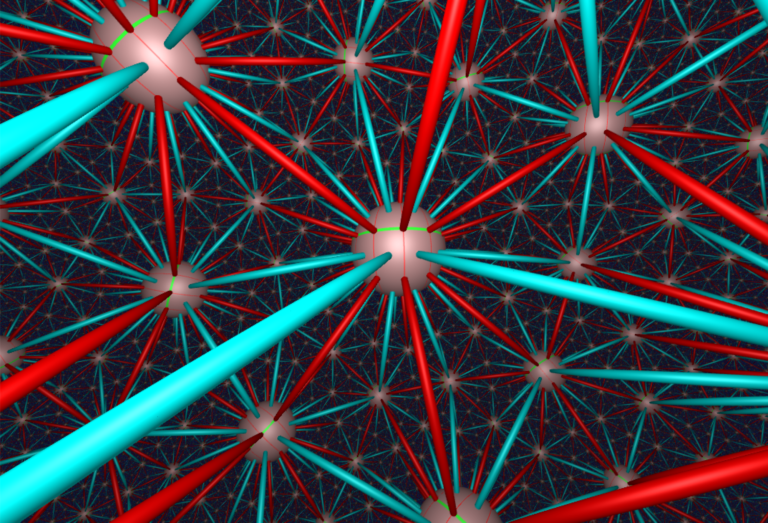
\includegraphics[height=.35\textheight]{snappy1.png}\hfill
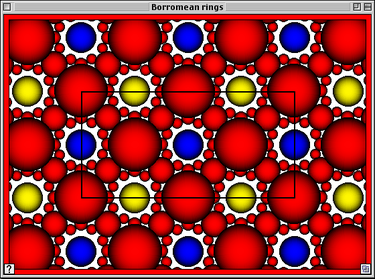
\includegraphics[height=.35\textheight]{SnapPea-horocusp_view.png}
}
\vspace{1.5cm}

\begin{itemize}
\item Spectre des longueurs combinatoire.
\item comptage de courbes simples (cf. CGAL)
\end{itemize}

\end{frame}
%---------------------------------------------------
\begin{frame}
  \frametitle{Graphe des pantalons et fonctions harmoniques}
  \centerline{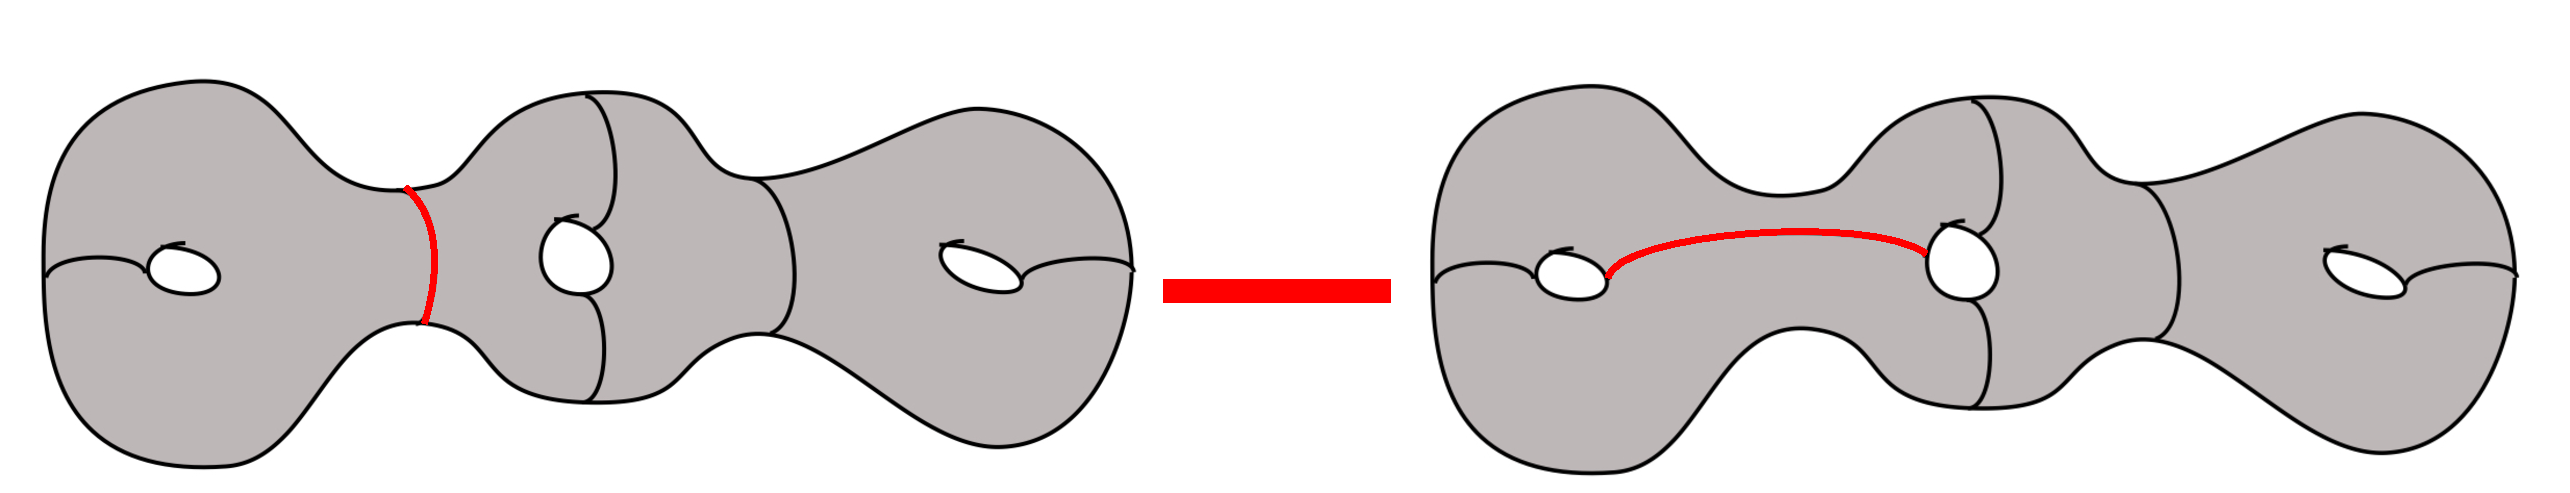
\includegraphics[width=\linewidth]{pants-graph.pdf}
  }
  \vspace{1.5cm}
  
  \begin{itemize}
  \item Extension de Flipper aux surfaces sans bord.
    \item Calcul d'invariants pour le mapping class group via son action sur le graphe des pantalons.
  \end{itemize}
\end{frame}
%---------------------------------------------------
\begin{frame}
  \frametitle{Structures géométriques}
\centerline{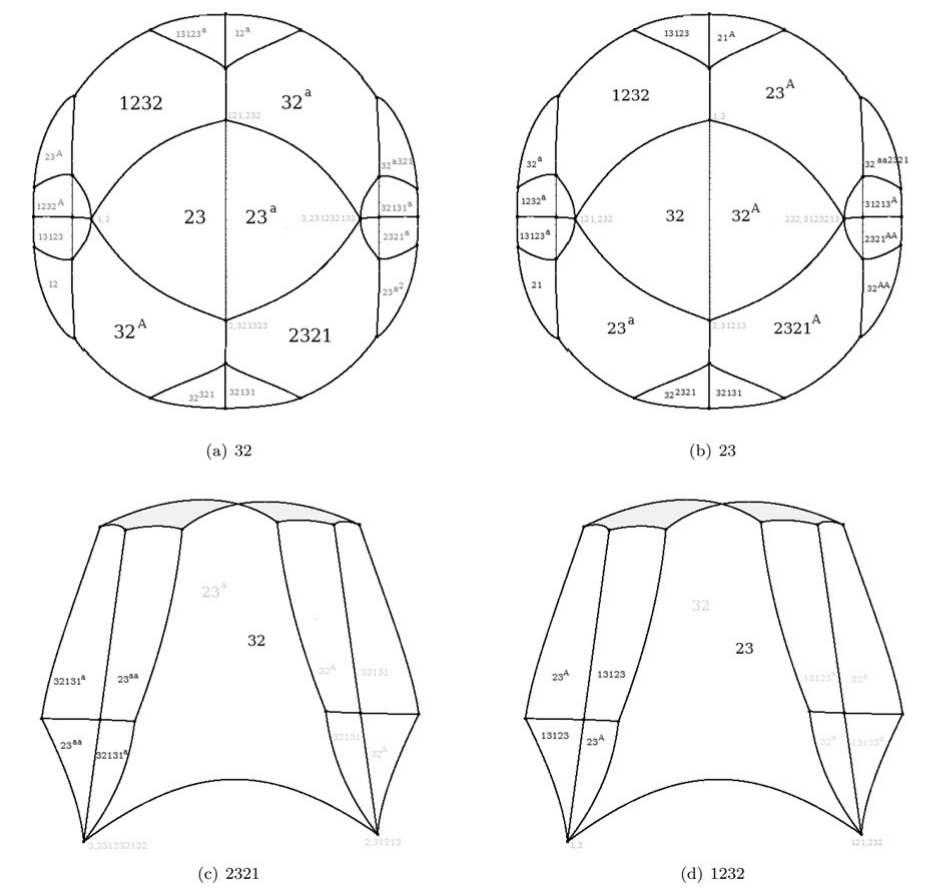
\includegraphics[width=.5\linewidth]{Ford-domain.png}
  }
  \begin{itemize}
  \item CR structures sur les variétés de dimension 3.
    \item Analogue de SnapPy pour les structures CR.
  \end{itemize}
\end{frame}
%---------------------------------------------------
\begin{frame}
  \frametitle{Bibliothèque dédiée aux courbes sur les surfaces}
\centerline{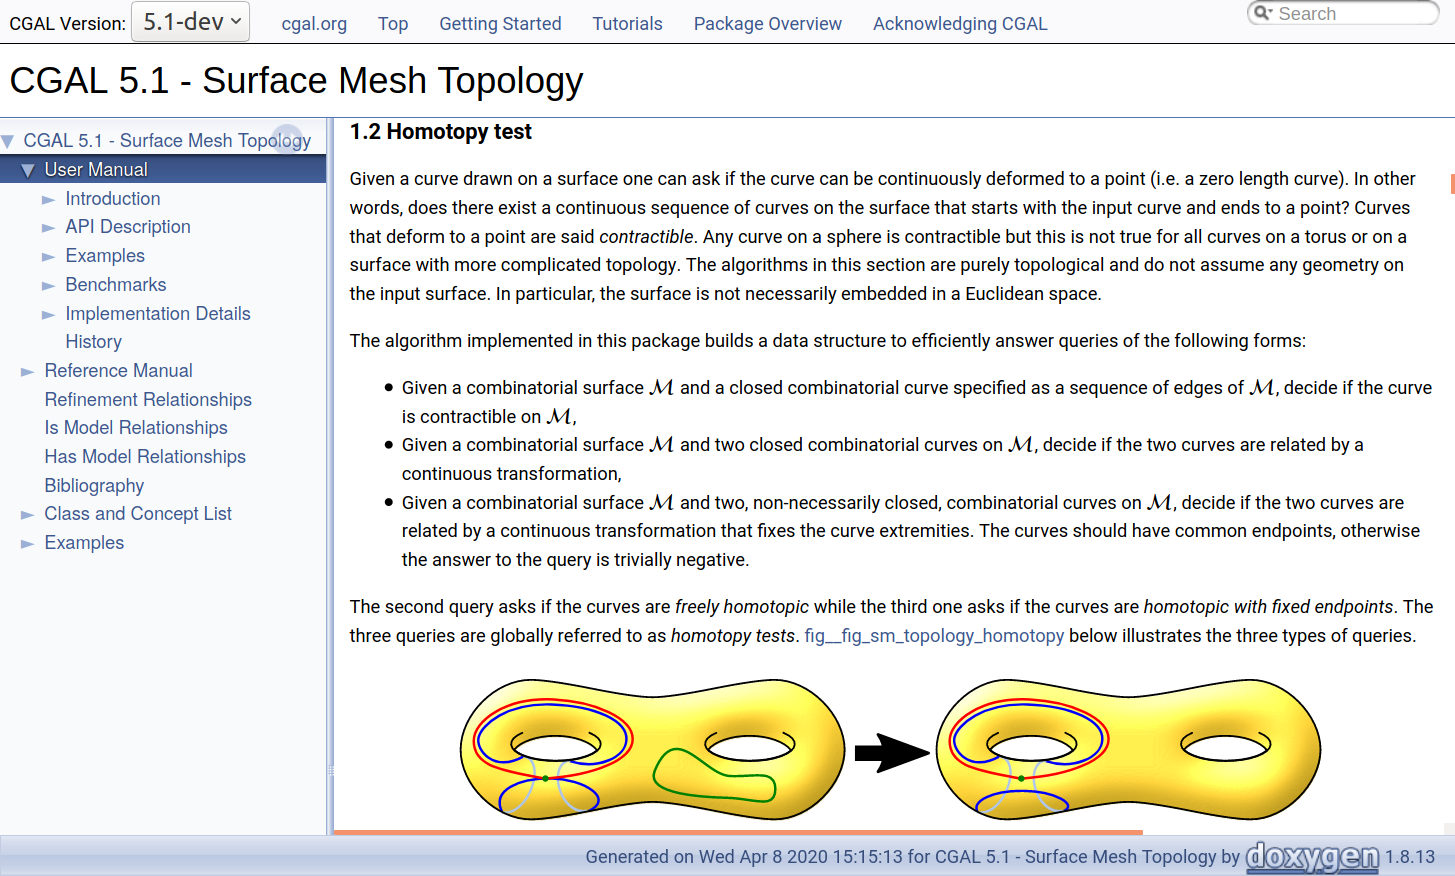
\includegraphics[height=.7\textheight]{CGAL_Surface_Mesh_Topology.png}}
\end{frame}
%---------------------------------------------------

\begin{frame}
  \frametitle{Activités et interactions}
  \begin{itemize}
  \item Groupe(s) de lecture (Matveev, ...)
    \item Développement logiciel open source (CGAL,...),
\item Invitations pour séminaires et cours doctoraux
\item colloques SMF-AMS
\item interactions européennes (Warwick, Luxembourg,...)
  \end{itemize}
\end{frame}
%---------------------------------------------------
\begin{frame}
  \frametitle{Diffusion}
\centerline{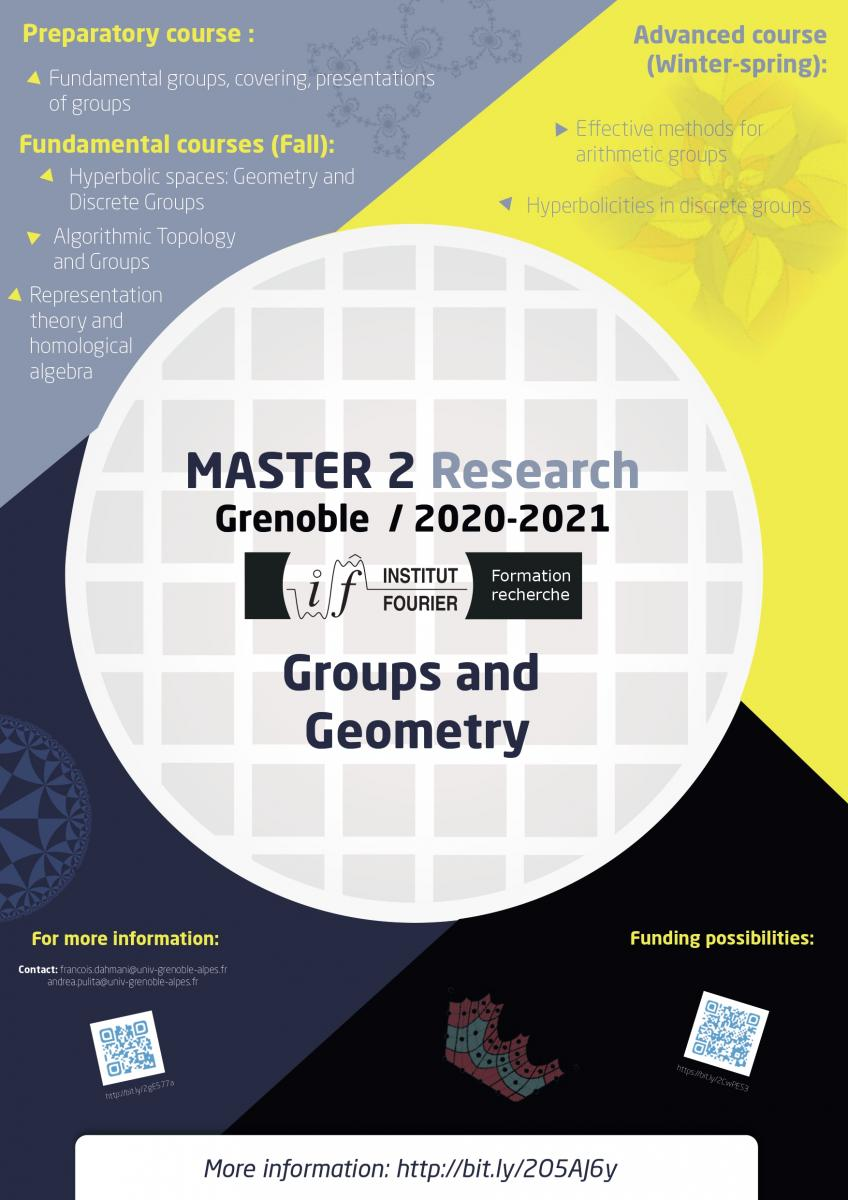
\includegraphics[height=.8\textheight]{POSTER-20-21.jpg}%{masterM2R_anglais_2020.pdf}
}
\centerline{\href{https://www-fourier.ujf-grenoble.fr/m2r/}{https://www-fourier.ujf-grenoble.fr/m2r/}}
\end{frame}
%---------------------------------------------------
\begin{frame}
  \frametitle{Demande de moyens}
\begin{itemize}
\item[] {\bf Financement de thèse} : \hfill 100.000 \EUR\\
\item[] {\bf Post-doc} (1 an) : \hfill 50.000 \EUR\\
\item[] {\bf Gratifications de stage} : \hfill 6.000 \EUR\\
{\footnotesize correspondant à 3 stages M2 de 5 mois.}
\item[] {\bf Invitations de chercheurs extérieurs} : \hfill 6.000 \EUR\\
\item[] {\bf Missions} : \hfill 20.000 \EUR\\
{\footnotesize (1200\EUR par personne et par an)}
\item[] {\bf Matériel} : \hfill 4.000 \EUR
\item[] {\bf Fonctionnement} : \hfill 4.000 \EUR
\item[] {\bf Congrès-colloques} : \hfill 10.000 \EUR
\item[] \rule[-0.1cm]{\linewidth}{0.01cm} 
\item[] {\bf TOTAL demandé : \hfill 200.000 \EUR}
\end{itemize}
\end{frame}
%---------------------------------------------------
\end{document}
%---------------------------------------------------
\begin{frame}
  \frametitle{}
\end{frame}
